%!TEX root = /Users/markelikalderon/Documents/Git/timaeus/timaeus.tex

\chapter{Cognitive Revolution} % (fold)
\label{cha:cognitive_revolution}

\section{Psychogeny and Cognitive Power} % (fold)
\label{sec:psychogeny_and_psychic_power}

The psychogeny, understood strictly as Timaeus' account of the generation of the World-Soul, was the topic of the last chapter. Timaeus' account of the generation of the World-Soul is important since the nature of its substance, its proportional division, and its being formed into the Circles of the Same and the Different determine its kinetic and cognitive powers. Our understanding of these powers is incomplete unless they are understood to be determined, at least in part, by the substance, proportional division, and structure that the World-Soul has thanks to Demiurgic activity. The details of the Demiurge's manufacture and construction of the World-Soul thus go some way to explaining the powers that He invests it with. Timaeus makes this connection explicit with respect to its cognitive powers. The World-Soul has its cognitive powers inasmuch as it is a mixture of Being, Sameness, and Difference, proportionally divided, and revolves around itself (37a). The explanation of the exercise of the World-Soul's cognitive powers would thus involve its substance, proportional division, and structure.

The World-Soul is elder sister to the souls of mortal beings. The Demiurge is the maker and Father of the World-Soul as well as the souls of mortal beings. The souls of mortal beings are generated after the generation of the World-Soul. The souls of mortal beings are mixed from the same material, though impurely, that was used to mix the substance of the World-Soul. Moreover, the Demiurge invests the souls of mortal beings with the same proportional divisions and structure as the World-Soul. The World-Soul is prior not only in birth but in dignity. It is more perfect than the souls of mortal beings as signaled by the impurity of their substance. Being perfect it is an exemplar for the souls of mortal beings. Thus like an elder sister, the souls of mortal beings look to her for guidance. Literally. The cognitive powers of the World-Soul are visibly manifest in the harmony of celestial motion. And by rationally attending to this motion in the right sort of way the circles in the souls of mortal beings are aligned to the circles in the World-Soul making them more rational and virtuous. In this way should we strive to be like our elder sister.

The way that the psychogeny explains the exercise of the cognitive powers of the World-Soul is relevant to the psychology of mortal beings. Given the relationship between the World-Soul and the souls of mortal beings, the explanation of the exercise of the cognitive powers of the souls of mortal beings should parallel the explanation of the exercise of the cognitive powers of the World-Soul. 

This chapter will discuss the cognitive powers of the World-Soul as Timaeus presents them to be at 37a--c. The passage largely consists in two long and syntactically complex sentences that have been variously interpreted. There Timaeus describes:
\begin{enumerate}[(1)]
	\item The objects of these cognitive powers, divisible and indivisible beings
	\item The World-Soul's ``contact'' (\emph{ephaptētai}) with its objects
	\item The cognitive activity that ``contact'' elicits
	\item The two kinds of cognitive powers that the World-Soul enjoys, the power to understand and know the indivisible and the power to have true opinion and conviction about the divisible.
\end{enumerate}
Let us consider these in turn.

% section psychogeny_and_psychic_power (end)

\section{The Objects of Cognition} % (fold)
\label{sec:the_objects_of_cognition}

The objects of cognition have either divisible or indivisible Being. Divisible Being is associated with Becoming (\emph{gignomenēs}) and is divided around bodies (\emph{peri ta somata} \ldots\ \emph{meristēs}), whereas indivisible Being always remains the same (\emph{aei kata tauta}). Being divided around bodies, divisible Being is corporeal. And since the sensible is the mark of the corporeal, divisible beings are sensible. Indivisible beings, by contrast, are not divided around bodies, and so are not sensible and corporeal, but are, rather, intelligible.

How is this related to the psychogeny? Timaeus specifies the different kinds of objects of cognition in terms a difference in their Being. One kind enjoys indivisible Being, and the other suffers divisible Being. Being is mixed into the substance of the World-Soul. And though Timaeus does not make this explicit in his summary statement of the soul mixture at 37a, this involved mixing indivisible and divisible Being. That the substance of the World-Soul consists in a mixture of divisible and indivisible Being perhaps explains, at least in part, that the objects of its cognition are either divisible or indivisible beings. If so, perhaps Timaeus subscribes, as Aristotle (\emph{De anima} 1 2 404b) suggest, to some version of the principle that like is known by like. 

It will emerge that different cognitive powers are exercised on the different objects of cognition. The World-Soul knows indivisible beings and has true opinions about divisible beings. The stability of indivisible beings, that they always remain the same, make them appropriate objects of knowledge. Whereas the instability of divisible beings, belonging to the realm of Becoming, makes them at best the objects of true opinion.

% section the_objects_of_cognition (end)

\section{\emph{Ephaptētai}} % (fold)
\label{sec:_emph_ephatetai}

The World-Soul is in ``contact'' (\emph{ephaptētai}) with the objects of cognition, be they divisible or indivisible, sensible or intelligible. As a result of this, the World-Soul is moved throughout the whole of its being and so announces what it is in contact with. How one understands \emph{ephaptētai} potentially constrains how one understands the motion of the World-Soul throughout the whole of its being by which it announces the object of its cognition. 

So far I have followed the bloodless convention of translating the verb \emph{ephaptētai} as a kind of contact. That verb, however, has a range of uses. The different senses conveyed by these may prove relevant. Let us begin by reviewing at least some of these.

In a range of uses the verb is used to convey \emph{binding}, somehow \emph{fixing} or \emph{holding fast} (Homer, \emph{Odyssey} 22 41). Observe that the emphasis is on the activity of binding rather than on the state of being bound. In another range of uses the verb has more tactile associations. It may be used to convey \emph{reaching} (Euripides, \emph{Helen} 556) or \emph{laying hands on} (Homer, \emph{Odyssey} 5 348). This second range of uses also emphasizes the bodily activity of the subject of the verb. Reaching and laying hands on are bodily activities. They are something done by embodied mortal beings embedded in an environment. They \emph{apply themselves} to that environment (Pindar, \emph{Olympian} 1 186). Moreover, reaching is an exploratory activity in a way that laying hands on may at least sometimes be (\citealt[134]{Betegh:2019fq}, emphasizes this aspect of \emph{ephaptētai}'s usage). The senses associated with these different uses need not conflict. Indeed, they may combine. Thus, for example, \emph{grasping} involves reaching and is a way to lay hands on something, but it also binds what is in its grasp. The verb has gustatory uses that emphasize not binding so much as assimilation, as when one \emph{partakes} of food (Iamblichus, \emph{Vita Pythagorae} 3 17). The verb also has purely cognitive uses that designate a kind of cognitive \emph{apprehension} (Plato, \emph{Symposium} 212a). (For discussion of a similar semantic field associated with perceptual apprehension see \citealt[chapters 1--2]{Kalderon:2018oe})

\citet[134]{Betegh:2019fq} has argued that the present occurrence of \emph{ephaptētai} must itself be understood in an active sense. The usual bloodless translation where the World-Soul is in contact with divisible and indivisible beings obscures the activity conveyed by the Greek. The World-Soul instead applies itself to divisible and indivisible beings. Reaching out and grasping is an apt metaphor for the World-Soul's cognitive apprehension of divisible and indivisible being. Cognitive apprehension is the World-Soul's activity, the way grasping is an activity. And, insofar as the object is apprehended, it is apt to think of this as a kind of binding, as when something is bound in one's grasp. And this remains true even when the binding could not be corporeal the way a grasping must be. 

Perhaps there are echoes of the other senses as well. The soul, in thinking, applies itself to the object of thought. Perhaps the soul in applying itself to divisible or indivisible being assimilates to these. In applying itself to the object of thought the soul partakes of what it thinks and becomes like it, in some suitable sense. This might be manifest in the ethical challenges that Timaeus understands the sensible to pose. But more compellingly, Timaeus' sensory soteriology presupposes something like the mortal soul' ability to assimilate to the object of its contemplation. The young gods, acting on the Demiurge's behest, providentially provide mortal beings with eyes to see with. In rationally attending to the harmony of celestial revolutions, the mortal being may align the circles in their soul with the circles in the World-Soul. Providentially provided sight is a means of salvation only insofar as it is a means by which the souls of mortal beings may assimilate to the soul of a divine immortal being and so become like their elder sister, insofar as that is possible.

To understand what \emph{ephaptētai} means in this context, let us begin by considering an obvious hypothesis about a special case. Begin by considering the special case where the World-Soul applies itself to a divisible being and, hence, to something sensible and corporeal. Since the object of cognition is sensible and corporeal, it is natural to consider whether \emph{ephaptētai} might involve a kind of corporeal contact. The tactile imagery conveyed by some uses of the verb---reaching, laying hands on---may suggest this. (Aristotle, \emph{De anima} 1 3 407a, reads Timaeus this way, for discussion see \citealt[392--5, 404--7]{Cherniss:1944aa} and \citealt[82--6]{Lee:1976xs}.) Just as a body may set into motion another body by coming into contact with it, perhaps the sensible and corporeal object of cognition sets the World-Soul into motion in just the same way. When the World-Soul applies itself to its corporeal object, this causes it to move throughout its whole being. The World-Soul is said not merely to move, but to move throughout its whole being. How are we to understand this qualification? The World-Soul, though incorporeal, is conceived as a sphere. Perhaps circular motion such as axial rotation would be a way for a sphere to move throughout its whole being. Beginning with our assumption that \emph{ephaptētai} involves corporeal contact, we were led to conceive of the resulting motion as the axial rotation of a sphere. This could only be so if the World-Soul were spatial. Only spatial things are spherical. Importantly, the World-Soul is also set into motion as a result of its contact with the divisible being, making the axial rotation subject to mechanical explanation.

There are difficulties in understanding \emph{ephaptētai} as corporeal contact, however. One potential difficulty concerns the mechanical explanation of the motion of the World-Soul. Doing so requires the corporeal object to be solid and offer resistance, and the incorporeal soul to itself be solid in order to be moved by contact with the corporeal object (\citealt[129--33]{Betegh:2019fq}). The potential problem is that solidity, on some understanding of that notion, is a condition on the possibility of touch (see chapter~\ref{sec:the_elemental_composition_of_the_corporeal}). If the solidity of the extended if incorporeal soul is suitably understood, then while the World-Soul may be invisible, it is tangible. When Timaeus claims that the World-Soul is invisible (36e), does he allow for this? Is it really plausible that the World-Soul may be felt if unseen? Or is invisible (\emph{aoratos}) a metonym for insensible, in which case the World-Soul is intangible? That Timaeus thinks visibility and tangibility to be opposed extremes of the sensible provides some support for the more general reading (Proclus, \emph{In Timaeum} 2 6--7, \citealt{Diehl:1903re}, see also Calcidius' translation of 31c as well as his \emph{In Timaeum} 21, discussed in chapter~\ref{sec:the_elemental_composition_of_the_corporeal}). If the World-Soul is insensible, it is intangible, and so not solid in the way required by the mechanical explanation of cognition. 

Johansen is sensitive to the problem and is led thereby to deny that the World-Soul is solid. Johansen observes that the sensible is the mark of the corporeal and that soul is insensible. Since the World-Soul is insensible, it is intangible. And since it is intangible, the World-Soul lacks the features that would make it tangible. Consider now not static touch, passively resting one's hand on an independently supported corporeal surface, but reaching out and grasping a body. What would a body have to be like to be tangible in this way. It would have to have depth and solidity. Anything that lacks depth would elude our grasp, and in grasping something with depth, it offers resistance to our grasp. And by experiencing this resistance we can have a sense of the overall shape and volume of the body in our grasp. Marking the sensible--insensible contrast thus involves making different spatial attributions to bodies and souls. Only bodies have depth and solidity as required for their tangibility in a way that our souls do not.

Part of the charm of the corporeal understanding \emph{ephaptētai} in the special case where the World-Soul applies itself to a divisible being is that it provides the resources for a mechanical explanation of the World-Soul's opinion about the sensible. In applying itself to divisible being, the World-Soul is in corporeal contact with its object and this causes it to engage in axial rotation. The mechanical explanation exploits the spatial character of the World-Soul. The World-Soul does occupy the space of the Cosmos---it is stretched throughout that space. But perhaps it does not occupy space in the same way as the body of the Cosmos. Something like the following thought might have motivated Johansen: If the World-Soul had depth an solidity, it would exclude the body of the Cosmos from occupying the same space. However, if the World-Soul lacks depth and solidity, it may spatially overlap the body of the Cosmos. Johansen is right to insist that whereas the corporeal is tangible, the World-Soul is intangible. What Johansen failed to see was that the World-Soul must meet the requirements on tangibility if the mechanical explanation of the soul's movement succeeds on its own terms. In order to move the soul, the divisible being must resist the soul's application to it. But such resistance is only possible if the World-Soul is itself solid. It is difficult to understand how the mechanical explanation of the World-Soul's opining could be consistent the sensible being the mark of the corporeal, the conditions on tangibility, and the World-Soul being insensible.

There are other difficulties with the mechanical explanation. Following \citet{Betegh:2019fq} we have retained an active sense for \emph{ephaptētai}. The present interpretation may have the World-Soul in corporeal contact with divisible being, but only by the World-Soul seeking out such contact. Still, the World-Soul's applying itself to the divisible being merely makes it a passive recipient of imparted motion. Even if the World-Soul only has the power to receive such motion if it actively applies itself to the sensible and the corporeal, there are elements of the passage that suggests that the World-Soul is the initiator of that movement and not merely its recipient. On the present interpretation, the opinion, the soul's announcement concerning the divisible being that it applies itself to, is the World-Soul's motion throughout its whole being that results from that contact. But later, Timaeus will speak of the announcement as being born through the self-moved. This suggests that the World-Soul, in applying itself to a divisible being, moves itself and is not itself moved in reaction to the encounter. If the World-Soul moves itself and is not moved by its encounter with a divisible being, then it is not a passive recipient of motion in the way that it would have to be if it were subject to the envisaged mechanical explanation. 

Even if this interpretation, or some variant of it, succeeds perfectly on its own terms, its ambitions are limited, and this, in the end, is its ruin. It only considers a special case, the World-Soul's applying itself to a divisible being. The World-Soul also applies itself to indivisible beings, intelligible beings such as the Forms. There is no question of conceiving the World-Soul's applying itself to the Forms as corporeal contact. Indivisible beings are not only incorporeal but inextended as well. And since only extended things may be solid, indivisible beings are not solid and so offer no resistance in corporeal contact. Either contact means different things when the World-Soul is said to be in contact with divisible Being and when it is said to be in contact with indivisible Being, or contact means something sufficiently general to cover both cases. Put another way, does \emph{ephaptētai} admit of homonymous or non-homonymous reading? Insisting that \emph{ephaptētai} be read as corporeal contact when applied to divisible beings commits one to a homonymous reading of \emph{ephaptētai}. Unfortunately, the homonymous reading does not cohere with the text.

Consider, then, a homonymous reading of \emph{ephaptētai}. When applied to divisible being it denotes a kind of corporeal contact. When applied to indivisible being it denotes a kind of non-corporeal contact. One problem with the homonymous interpretations of \emph{ephaptētai} is the grammatical context of its occurrence. It occurs in a context where we are being asked to consider the World-Soul applying itself to either a divisible or indivisible being. The homonymous reading should rule out such constructions. Either reading of \emph{ephaptētai}, as involving corporeal contact or not, would rule out the intelligible occurrence of one of its objects  (compare the standard linguistic tests for lexical ambiguity, \citealt{Zwicky:1975hl}). If \emph{ephaptētai} is interpreted as involving corporeal contact, while taking a divisible being as its objects is intelligible, taking an indivisible being as its object is not. And if \emph{ephaptētai} is interpreted as involving non-corporeal contact, while taking an indivisible being as its object is intelligible, taking a divisible being as its object is not. Such a construction could only be intelligible on a non-homonymous reading of \emph{ephaptētai}. The verb must mean something sufficiently general to intelligibly apply to both divisible and indivisible beings.

The homonymous reading of \emph{ephaptētai} is, if not incoherent, then inconsistent with the text. As a consequence, one should not understand the World-Soul's applying itself to divisible being as corporeal contact. Whatever the occurrence of the verb means, it must mean something sufficiently general to apply to sensible and intelligible objects, and it does not on the corporeal interpretation. 

Of its range of uses perhaps only its cognitive uses are sufficiently general on a literal interpretation of them (for example, Plato, \emph{Symposium} 212a; though such cognitive uses, literally understood, are surely dead metaphors). One obstacle to this suggestion is that the most straightforward understanding of it as false. So consider those uses where \emph{ephaptētai} means something like cognitive apprehension. The activity conveyed by \emph{ephaptētai} may be a part of the apprehension of a sensible object in opinion but it is not the whole of it. Opining involves not only the World-Soul applying itself to a sensible object, but moving itself throughout the whole of its being in response. So if \emph{ephaptētai} receives a cognitive reading, it must be less than the whole cognitive act effected, opining as applied to sensible objects and knowing as applied to intelligible objects. 

Perhaps \emph{ephaptētai} admits of a restricted cognitive reading. Perhaps \emph{ephaptētai} might be understood as analogous to attentive contact, an attentive contact involved in, if distinct, from the cognitive act. (I stress the analogy here. \emph{Ephaptētai} is not attentive contact it is merely like it. A conception of attention as an independent cognitive activity, though Platonic in its sources, is plausibly post-Timaean. Such a conception only fully emerges in the work of Plotinus and Augustine. The analogy only attributes to Timaeus an anticipatory trace of this post-Timaean idea.) Attending to a sensible object is not to opine about it. Nevertheless, in attending to a sensible object, the World-Soul moves itself throughout its whole being thus announcing the character of the sensible object attended to. Similar remarks apply to the intelligible case. Attending to intelligible objects is not yet to know them. Perhaps they must be brought into relation with other intelligible objects over the course of dialectic before they are truly known. And yet one only comes to know the intelligible by attending to it. In attending to an intelligible object, the World-Soul moves itself throughout its whole being thus announcing the character of the intelligible object attended to. So perhaps only a restricted cognitive reading of \emph{ephaptētai} is sufficiently general to cover the World-Soul's application to divisible and indivisible being. So interpreted, \emph{ephaptētai} is a kind of pre-cognitive attentive contact at work whenever the World-Soul cognizes.

There is a problem, however. While pre-cognitive attentive contact is less than the full cognitive act as required, it still does more than it should. On the present interpretation, attending to divisible or indivisible being fixes the intentional object of the cognitive act. But plausibly the intentional object of the cognitive act is only fully determined by the World-Soul moving itself throughout the whole of its being (a problem shared with Aristotle's corporeal reading of \emph{ephaptētai}, \emph{De anima} 1 3 407a18--9, \citealt[84, 98--9 n26]{Lee:1976xs}). Consistent with a restricted cognitive reading, \emph{ephaptētai} is better understood as a kind of pre-noetic orientation toward the intentional object of the cognitive act. It is analogous to reaching in the act of grasping. (\citealt[276]{Ross:1906fk}, and \citealt[404 n335]{Cherniss:1944aa}, take Aristotle's description of ``reaching out'' in thought in \emph{De memoria} 2 452b9--11 to be a reference to the present passage.) In reaching for something one does not grasp it. A body is the object of one's grasp only when one conforms one's hands to its contours and so binds it in one's grasp. Nevertheless, in reaching for a body one is orienting one's own body towards it in such a way that one may come to grasp it. It is part of the process of coming to grasp the body and not itself the grasping of it. Such a pre-noetic orientation is less than the full cognitive act as required. And while it may help determine the intentional object of the cognitive act, it does so consistent with that object only being fully determined by the World-Soul moving itself throughout the whole of its being. I shall henceforth speak of this pre-noetic orientation as the World-Soul applying itself to the object of its cognition.


% section _emph_ephatetai (end)

\section{Cognitive Activity} % (fold)
\label{sec:cognition}

Timaeus conceives of cognitive activity, the exercise of the World-Soul's cognitive powers, as an internal discourse. In cognizing, the truth about the objects of cognition are announced. Timaeus initially provides a general description of cognitive activity. His general description applies to the cognition of divisible as well as indivisible beings. Only subsequently does Timaeus discuss how the cognition of divisible beings may differ from the cognition of indivisible beings. (We shall take up this difference in section~\ref{sec:knowledge_and_opinion}.) In Peripatetic terms, Timaeus first describes the genus of cognitive activity before describing its species.

The World-Soul applies itself to divisible or indivisible beings. On a restricted cognitive reading of \emph{ephaptētai}, this is a kind of pre-noetic orientation toward the object of cognition. In applying itself to the divisible or indivisible beings, the World-Soul moves throughout the whole of its being and announces the character of the object applied to. The announcement, without speech or sound, is the cognitive act, the exercise of the Word-Soul's cognitive powers. A question immediately arises. Is the movement throughout the whole of its being the same as the announcement? Or is the movement merely a phase in the causal process eventuating in cognition? Porphyry attributes the latter interpretation to Amelius who held that the announcement was made only once the World-Soul ceased to move (\emph{In Timaeum} 74, \citealt{Sodano:1964mf} = Proclus, \emph{In Timaeum} 2 300.34--301.2, \citealt{Diehl:1903re}). Does the movement constitute the announcement or merely cause it?

Identifying the movement with the announcement is in one way parsimonious. Timaeus does not then have to provide a further account of what this announcement is. Though some explanation is owed as to how and in what sense this motion is an announcement. Indeed, this puts an important constraint on any such identification. The movement must be understood in such a way that it is intelligibly an announcement. If the movement could not be understood in this way, then that would be good reason to regard the movement as merely a phase in the causal process eventuating in cognition, in which case Amelius would be vindicated. The identity or difference of movement and announcement is only settled once we have a better understanding of the potential cognitive significance of the World-Soul moving itself throughout the whole of its being.

Let us begin with the movement of the World-Soul. The movement of the World-Soul is active. The World-Soul moves itself and is not itself moved in response to its application to its object. The World-Soul is a self-mover (\emph{kinoumenō huph autou}) and so is not moved by coming into contact with its object. It is not the passive recipient of motion but the initiator of the motion. The movement is the activity of the World-Soul. It rouses itself to this activity in applying itself to divisible or indivisible beings. The movement is less a mechanical effect than the arousal of a living being.

That the movement is not passively received but initiated by the World-Soul itself makes it akin to cognition in at least one respect. Thinking is not something done to a thinker, but something a thinker does. The movement throughout the whole of its being is like thinking in not being passively received but actively performed by the World-Soul. In Kantian parlance, it shares in the spontaneity of judgment.

There is some evidence that the movement throughout the whole being of the World-Soul is not only active but discursively structured. If the movement is discursively structured, it may intelligibly be an announcement, in which case movement and announcement may be identified. Timaeus comes close to explicitly claiming as much when he tells us that the announcement is born through the self-moved without speech or sound (37b5--7). It is at least natural to suppose that the announcement is born through the self-moved by the World-Soul moving itself throughout its whole being constituting the announcement. The World-Soul is not merely the audience of the announcement but its author. Thinking, here, is being envisaged as the soul's conversation with itself. This is, of course, a familiar Platonic theme. (Compare \emph{Theaetetus} 190a and \emph{Sophist} 263e, 264a--b.) Even if the announcement being born through the self-moved provides some evidence that the self-initiated movement is discursively structured, it does not yet explain how it might be.

To get a better sense of how the active motion may be discursively structured, we shall consider the account of discursive structure offered in the \emph{Sophist} (260a--263e). Doing so shall highlight aspects of the present passage whose significance might otherwise go unnoticed. Importantly, I shall not insist on doctrinal uniformity between the \emph{Timaeus} and the \emph{Sophist}. Moreover, there are real differences in emphasis. In the \emph{Sophist}, the Eleatic Stranger is concerned to establish the possibility of false statements, whereas Timaeus is describing the true opinion and knowledge of the World-Soul. The possibility of error is something only the younger siblings of the World-Soul, the souls of mortal beings, must grapple with. (On the Eleatic Stranger on discursive structure see \citealt[]{Frede:1992ec}, on its relation to the \emph{Timaeus} see \citealt[]{Betegh:2019fq}.)

According to the Eleatic Stranger, making a statement requires two things. The speaker must first identify the subject of the statement, what they want to make a statement about, but they must also second specify what is said about the subject. Thus a statement must at least contain two parts, a part identifying the subject of the statement and a part specifying what that statement says of the subject. The former is a noun and the latter is a verb. To make a statement, a speaker must ``weave'' together the noun and the verb. Philoponus' take on interweaving might be appropriate here as well. The interweaving of noun and verb in making a statement is neither their fusion nor mere juxtaposition. The interweaving of noun and verb is not a fusion since statements admit of decomposition into nouns and verbs and so are intelligibly differentiated. And the interweaving is not merely juxtaposition since not all juxtapositions of words make meaningful statements (\emph{Sophist} 263d). The interweaving of noun and verb is such that what is specified by the latter is related to what is identified by the former. There are two kinds of statements, affirmative and negative statements. Affirmative statements say that the same are the same and negative statements say that the different are different. If what the noun applies to is different from what is specified by the verb, then different things are said as the same and the affirmative statement is false (\emph{Sophist} 263d). Conversely, if what the noun applies to is the same as what is specified by the verb, then the affirmative statement is true. Finally, reasoning is understood as the soul's conversation with itself and opinion (\emph{doxa}) is the result of this conversation (\emph{Sophist} 264a--b). Cognition, conceived as a kind of inner speech, must similarly display this discursive structure.

The Eleatic Stranger's discussion of the soul's conversation with itself (\emph{Sophist} 264a--b) introduces a potential complexity. There the soul's conversation with itself is understood as reasoning, the rational process by which judgment is fixed, and its result is cognition. Applying this idea to Timaeus' speech might suggest that the World-Soul moving itself throughout its whole being is the process by which cognition is fixed and the announcement the result. This would be to revive Amelius' interpretation. If, however, the announcement being born through the self-moved is explained by the announcement just being the self-initiated movement, then Amelius' interpretation should be rejected, and the Eleatic Stranger's account not applied in this manner to Timaeus' speech. If anything, it is (\emph{ephaptētai}) that describes a phase in the process of fixing cognition.

The World-Soul applies itself to (\emph{ephaptētai}) divisible and indivisible beings. On a restricted cognitive reading this is a pre-noetic orientation to the object of cognition. The identification of the object of cognition is only complete with the circular motion of the World-Soul. So this is best understood as the process of coming to identify what the cognitive act is about. The object of cognition is the subject of inner speech. It is what the announcement is about. The announcement says something about its subject, the object of cognition. If the subject of the announcement is the same as what the announcement says of it, then the announcement is true. The World-Soul only makes true announcements, and the two kinds of announcements that it makes corresponds to the two kinds of statements that may be made in speech. True statements are either affirmative or negative, they either say that the same are the same or that the different are different. And this is what the World-Soul's announcements do, they say that the same are the same and that the different are different (37).

Those commentators that see Timaeus, here, as subscribing to the principle that like is know by like make a connection between the cognitive activity of saying that the same is the same and the different is different with the World-Soul being composed of a mixture of Being, Sameness, and Difference. Being composed, in part, of Sameness, the World-Soul is capable of judging the same as the same. And being composed, in part, of Difference, the World-Soul is capable of judging the different as different. How must we conceive of this cognitive activity in order for this to be so? One way, perhaps not the only way, would be if the cognitive activity is the World-Soul moving itself throughout its whole being, a being composed of Sameness and Difference.

It is tempting to envision the movement by which the World-Soul announces the same as the same as the revolution of the Circle of the Same, and the movement by which the World-Soul announces the different as different as the revolution of the Circle of the Different. The temptation should be resisted. First, notice that Timaeus will subsequently distinguish knowledge and opinion in terms of these. Thus when the World-Soul applies itself to an indivisible being, something intelligible and incorporeal, the Circle of the Same revolves, and the World-Soul understands and knows its object. And when the World-Soul applies itself to a divisible being, something sensible and corporeal, the Circle of the Different revolves, and the World-Soul has true opinion and conviction about its object. Second, notice that the Circles of the Same and the Different are so called not because of any substantial difference between them. Each are composed of the same mixture Being, Sameness, and Difference and with the same proportional divisions. That means that the different revolutions of the circles in knowledge and opinion could not be explained in terms of a substantial difference since they share the same substance. The principle that like is known by like has no grip here. Moreover, indivisible beings are themselves the same or different from other indivisible beings. So it would be a mistake to think that knowledge only judges the same as the same, it judges the different as different as well. And it is thanks to the Circle of the Same being composed, in part, by Difference that it may announce the different as different even among the indivisible. Similarly, it is thanks the Circle of the Different being composed, in part, of Sameness that it may announce the same as the same even among the divisible. Both knowledge and opinion involve judging the same as the same and the different as different. Even the degraded form of cognition available to embodied mortal beings embedded in an environment, perception, involves not only discrimination but perceptual grouping as well, as when one succeeds in seeing the numeral in an Ishihara color test (see figure~\ref{fig:ishihara}). Timaeus does not ever explicitly identify the movement associated with announcing the same as the same and the different as the different.

\begin{figure}[htbp]
	\centering
		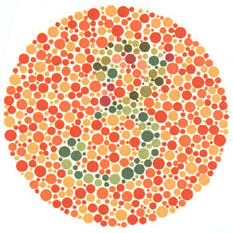
\includegraphics[scale=1.5]{graphics/ishihara.jpg}
	\caption{Ishihara Color Test}
	\label{fig:ishihara}
\end{figure}

We should not assume that the movement that constitutes the announcement is simple. The Demiurge has fabricated a complex structure for the World-Soul. He does so to invest the World-Soul with the power of complex motion. The greatness of this power is visibly manifest in the complexity of celestial motion. The assumption that the movement is simple motivates, in part, the temptation to identify judgements of Sameness with the revolutions of the Circle of the Same. If we abandon that assumption, new interpretative possibilities open up.

To appreciate this, indulge me, just for the moment, in a speculative take on the text. Consider the World-Soul applying itself to a divisible being and announcing its character in true opinion. Suppose the World-Soul applies itself to Theaetetus and so comes to cognize this divisible being. To cognize Theaeteus is to engage in circular motion. Since it is Theaetetus that is cognized, presumably he is at the center of this circular activity. That is what it means for a divisible being to be the object of cognition. In cognizing Theaetetus, the World-Soul recognizes his activity as sitting. To recognize Theaetetus' activity is itself to engage in circular motion. However, since the World-Soul is complex, we need not assume that it is the same circular motion as the one that cognizes Theaetetus. Not only has the Demiurge invested the World-Soul with a complex structure, he also imposed proportional divisions within its substance. And this opens up the possibility of understanding interweaving within Timaeus's \emph{eikos muthos}. Perhaps the two motions are interwoven in the sense that they are harmonious or attuned to the proportional divisions providentially established in the substance of the World-Soul. As on Philoponus' take on interweaving, the two circular motions are neither fused nor juxtaposed. They are not fused. The circular motions remain two and the movement constituting the announcement is complex. Nor need they be juxtaposed. Indeed what could juxtaposition even here mean? Interweaving is rather the harmony of their revolutions. On this interpretation, judging the same as the same is a complex motion involving two revolutions attuned to one another. The World-Soul's opinion consists in its moving itself throughout its whole being in this complex harmonious fashion. The interpretation is not only speculative, but incomplete insofar as no specific part of the complex structure has been identified as moving. 



% section cognition (end)

\section{Knowledge and Opinion} % (fold)
\label{sec:knowledge_and_opinion}



% section knowledge_and_opinion (end)

\section{Concluding Observations} % (fold)
\label{sec:concluding_observations_cr}



% section concluding_observations (end)

% chapter cognitive_revolution (end)